\documentclass[titlepage,12pt]{report}

\usepackage[utf8]{inputenc}
\usepackage[a4paper, total={6in, 8in},headheight=14pt]{geometry}
\usepackage{newtxtext,newtxmath}
\usepackage[scaled=1]{couriers}
\usepackage[spanish]{babel}
\usepackage{microtype}
\usepackage[bottom]{footmisc}
\usepackage{fancyhdr}
\usepackage{graphicx}
\usepackage{blindtext}
\usepackage{scrextend}
\usepackage{tocloft}
\usepackage{parskip}
\usepackage{multicol}
\usepackage{subcaption}
\usepackage{wrapfig}
\usepackage{multicol}
\usepackage{verbatimbox}
\usepackage[nottoc, notlot, notlof]{tocbibind}
\usepackage{listingsutf8}
\usepackage{url}
\usepackage[square,numbers]{natbib}
\usepackage{adjustbox}
\usepackage[makeroom]{cancel}
\usepackage[hidelinks]{hyperref}
\usepackage[Glenn]{fncychap}
\usepackage{lastpage}
\usepackage{fancyhdr}

\bibliographystyle{unsrtnat}

\pagestyle{fancy}
\fancyhf{}
\fancyhead[R]{\rightmark}
\fancyfoot[C]{\leftmark}
\fancyfoot[R]{\thepage}
\renewcommand{\footrulewidth}{0.6pt}% Line at the footer visible
\addto\captionscatalan{%
  \renewcommand\contentsname{Índice}%
}

\fancypagestyle{plain}{%
  \fancyhf{}%
  \fancyfoot[R]{\thepage}%
  \renewcommand{\headrulewidth}{0pt}% Line at the header invisible
  \renewcommand{\footrulewidth}{0.6pt}% Line at the footer visible
}


\renewcommand{\cftpartleader}{\cftdotfill{\cftdotsep}}%
\renewcommand{\cftsecleader}{\cftdotfill{\cftdotsep}}%
\renewcommand\familydefault{\sfdefault}

\usepackage{tikz}
\usetikzlibrary{shapes.geometric, arrows}

\newcommand{\Lagr}{\mathcal{L}}
\newcommand{\Xagr}{\mathcal{X}}

\setlength{\skip\footins}{1cm}

\makeatletter
% \patchcmd{<cmd>}{<search>}{<replace>}{<success>}{<failure>}
\patchcmd{\@makechapterhead}{\huge}{\large}{}{}% for \chapter
\patchcmd{\@makechapterhead}{\Huge}{\large}{}{}% for \chapter
\patchcmd{\@makeschapterhead}{\Huge}{\large}{}{}% for \chapter*
\makeatother


\begin{document}

\iftrue
\newcommand{\HRule}{\rule{\linewidth}{0.5mm}}

\thispagestyle{empty}

\begin{center}

{\large Universitat Politècnica de Catalunya}

\medskip
{\large Facultat d'Informàtica de Barcelona (FIB)}

\vfill
{\bfseries\Large Bachelor's Degree Project}

\vfill
\centerline{\mbox{
\includegraphics[width=60mm]{media/FIB_UPC.png}}}

\vfill
\vspace{5mm}

{\LARGE Jordi Gil González}

\vspace{15mm}

% Title in English according to the official assignment
{\LARGE\bfseries Analysis of the Path Tracing \\ rendering method on CPU and GPU}

\normalfont \small \sffamily{}

\vfill

Computer Science Department


\vfill

\begin{tabular}{rl}
Bachelor's Degree Project Director: & Chica Calaf, Antoni \\
\noalign{\vspace{2mm}}
Study programme: & Computer Science\\
\noalign{\vspace{2mm}}
Specialization: & Computer Graphics\\
\end{tabular}

\vfill

\large Academic Year 2019/2020

\large \today

\end{center}

\newpage
\tableofcontents*
\fi

\newpage

\chapter{Planificación temporal}

\section{Planificación y programación}

Este capítulo trata la planificación del proyecto y describe las tareas realizadas, a través de un plan de acción, para cumplir los plazos relativos a la entrega del proyecto. Veremos también los recursos utilizados y se tendrán en cuenta los posibles obstáculos que puedan modificar la planificación.

El proyecto se inició a principios de julio de 2019 con vista a entregarlo el 13 de enero de 2020.

\section{Descripción de tareas y recursos utilizados}

\subsection{Descripción de tareas}

\subsubsection{Estudio de conceptos}

Antes de comenzar el proyecto, fue necesario familiarizarse con los conceptos básicos que rigen nuestro proyecto. Durante el semestre previo hubo un par de reuniones con el director del proyecto para definir el tema en el cual se centraría y poder así encaminarlo. También, el autor del presente proyecto se matriculó de la asignatura de Tarjetas Gráficas y Aceleradores (TGA por sus siglas) para introducirse en la programación en el entorno de \texttt{CUDA} y así agilizar el proceso de desarrollo del proyecto su etapa inicial. Dado que esta tarea se realiza fuera del proyecto sumado a la dificultad de determinar una estimación en horas, no se tendrá en cuenta en la planificación.

\subsubsection{Configuración del sistema}

Antes de entrar propiamente en el desarrollo en si del proyecto, debemos configurar las herramientas necesarias y garantizar su correcto funcionamiento.

Para poder desarrollar el proyecto será necesario tener instalado en nuestros sistemas la API de \texttt{CUDA} con tal de poder crear el programa principal de nuestra aplicación paralela en GPU. Las librerías de \texttt{OpenMP} vienen instaladas por defecto en los sistemas Linux, por lo que no será necesaria una instalación, pero sí comprobar que funcionan correctamente. Por último, haremos uso de una plataforma, \textit{TexMaker}, que nos permita compilar código \LaTeX con tal de generar la documentación requerida.

Esta configuración debe hacerse tanto en el computador de sobremesa como en el portátil. La parte de \textit{CUDA} en el cluster de docencia no será necesario de configurar debido a que ya está previamente configurado por el DAC (Departament d'Arquitectura de Computadors). 

\subsubsection{Planificación del proyecto}

Esta es la tarea que se está desarrollando actualmente. Esencialmente trata sobre todo el contenido cubierto por el curso de GEP. La podemos dividir en tres subtareas:

\begin{enumerate}
		\item Contextualización y alcance.
		\item Planificación temporal.
		\item Presupuesto y sostenibilidad.
\end{enumerate}

\subsubsection{Desarrollo}

Esta tarea es la más importante de todo el proyecto. Cubre el desarrollo de las aplicaciones, experimentación y documentación de los resultados de cada una de las partes. Dividiremos el desarrollo en cuatro ciclos de 14 días cada uno, coincidiendo con las reuniones programadas con el director del presente proyecto. Cada uno de los ciclos los dividiremos en cuatro tareas:

\begin{itemize}

	\item \textbf{Desarrollo versión secuencial:} Se trata de la versión más básica de todas. Sirve como base para desarrollar tanto la versión paralela en CPU (\texttt{OpenMP}), como la versión paralela en GPU (\texttt{CUDA}).
	
	\item \textbf{Desarrollo versión paralela CPU:} Una vez implementada la versión secuencial pasaremos a implementar una versión paralela de ésta haciendo uso de la librería de \texttt{OpenMP}. 
	
	\item \textbf{Desarrollo versión paralela GPU:} Una vez implementada la versión secuencia pasaremos a implementar una versión paralela de ésta haciendo uso de \texttt{CUDA}.

	\item \textbf{Experimentación:} Crearemos la misma escena en cada una de las versiones comentadas en los puntos anteriores y analizaremos el rendimiento de ambas, teniendo en cuenta el tiempo de creación requerido para generar la imagen final.

\end{itemize}

Las dependencias entre las diferentes tareas son fáciles de describir. Hasta que no tengamos la versión secuencial no podremos empezar a programar las versiones paralelas de ésta. Tampoco podremos empezar un ciclo nuevo sin haber terminado el anterior.

\subsubsection{Etapa final}

En esta etapa estructuraremos toda la documentación de las etapas anteriores y preparemos la presentación final para la defensa del proyecto.

\subsection{Tabla resumen y Estimación}

\begin{table}[H]
	\centering
	\begin{tabular}{|m{5cm}||m{5cm}|}
		\hline
		Tarea & Tiempo empleado (horas) \\ \hline \hline
		Configuración del sistema & 10 \\ \hline
		Planificación del proyecto & 130 \\ \hline
		Desarrollo & 330 \\ \hline
		Etapa final & 120 \\ \hline \hline
		Total & 590 \\ \hline
	\end{tabular}
	\caption{Resumen de horas}
\end{table}

Con una estimación de 35 horas a la semana (3 horas de lunes a jueves, 10 horas sábados y domingos), y teniendo presentes un total de 18 semanas de trabajo, tenemos: $35h \cdot 18 = 630$ horas en total. Esto nos deja un margen de tiempo para posibles inconvenientes.

\subsection{Recursos utilizados}

\subsubsection{Software}

\begin{itemize}
	\item Linux, usado en todas las tareas.
	\item \LaTeX , para realizar la documentación.
	\item \texttt{C++},\texttt{OpenMP} y \texttt{CUDA}, para el desarrollo de las aplicaciones.
	\item \texttt{git}, utilizado para el control de versiones y compartir el código entre diferentes entornos (computador de sobremesa y el portátil).
\end{itemize}

\subsubsection{Hardware}

\begin{itemize}
	\item PC Sobremesa con las siguientes características: i7 7700 3.6 GHz, NVIDIA GeForce RTX 2080 SUPER, 24GB RAM, 250 SSD, 1TB SSD, 1TB HDD
	\item PC Portátil con las siguientes características: i7 7700HQ 2.8GHz, NVIDIA GeForce 1050 Mobile, 8GB RAM, 500GB SSD
	\item Cluster de docencia con las siguientes características: Intel Xeon E5-2620 v2 2.10GHz x2, NVIDIA Tesla K40c x4, 64GB RAM, 1TB x2
\end{itemize}

\section{Diagrama de Gannt}

\begin{figure}[H]
\centering
\begin{minipage}{.5\textwidth}
  \centering
  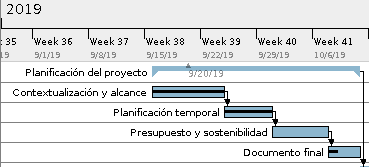
\includegraphics[scale=0.6]{media/gantt_1.png} %%width=.4\linewidth
  \captionof{figure}{Etapa de gestión. \\ Fuente: Creación propia}
  \label{gantt_1}
\end{minipage}%
\begin{minipage}{.5\textwidth}
  \centering
  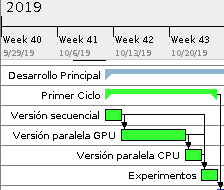
\includegraphics[scale=0.75]{media/gantt_2.png}
  \captionof{figure}{Primer ciclo. \\ Fuente: Creación propia}
  \label{gantt_2}
\end{minipage}
\end{figure}

\begin{figure}[H]
\centering
\begin{minipage}{.5\textwidth}
  \centering
  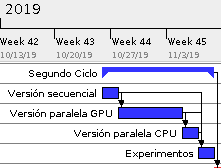
\includegraphics[scale=0.75]{media/gantt_3.png} %%width=.4\linewidth
  \captionof{figure}{Segundo Ciclo. \\ Fuente: Creación propia}
  \label{gantt_3}
\end{minipage}%
\begin{minipage}{.5\textwidth}
  \centering
  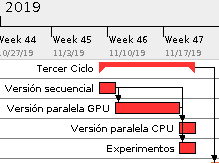
\includegraphics[scale=0.75]{media/gantt_4.png}
  \captionof{figure}{Tercer ciclo. \\ Fuente: Creación propia}
  \label{gantt_4}
\end{minipage}
\end{figure}

\begin{figure}[H]
\centering
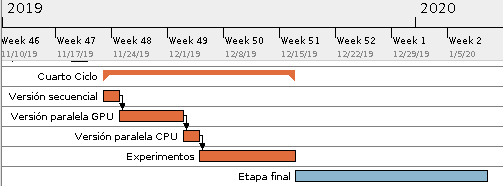
\includegraphics[scale=0.5]{media/gantt_5.png}
\captionof{figure}{Cuarto ciclo y etapa final. \\ Fuente: Creación propia}
\label{gantt_5}
\end{figure}

\section{Gestión de riesgos: Planes alternativos y obstáculos}

Como podemos observar en la Figura \ref{gantt_5}, en el cuarto ciclo de desarrollo la tarea de experimentos ocupa más tiempo en comparación a ciclos anteriores. En este caso, hemos sobrestimado la duración de ésta para tener tiempo suficiente de resolver problemas que puedan aparecer, como los definidos en el capítulo anterior (Contextualización y alcance), en el curso del desarrollo del proyecto o experimentos que puedan surgir a última hora. 

En el \textit{Anexo I} podremos ver una imagen del diagrama de Gannt completo.

\clearpage
\addappheadtotoc
\appendixpage

\chapter{Anexo I: Diagrama de Gantt}

\begin{figure}[H]
\centering
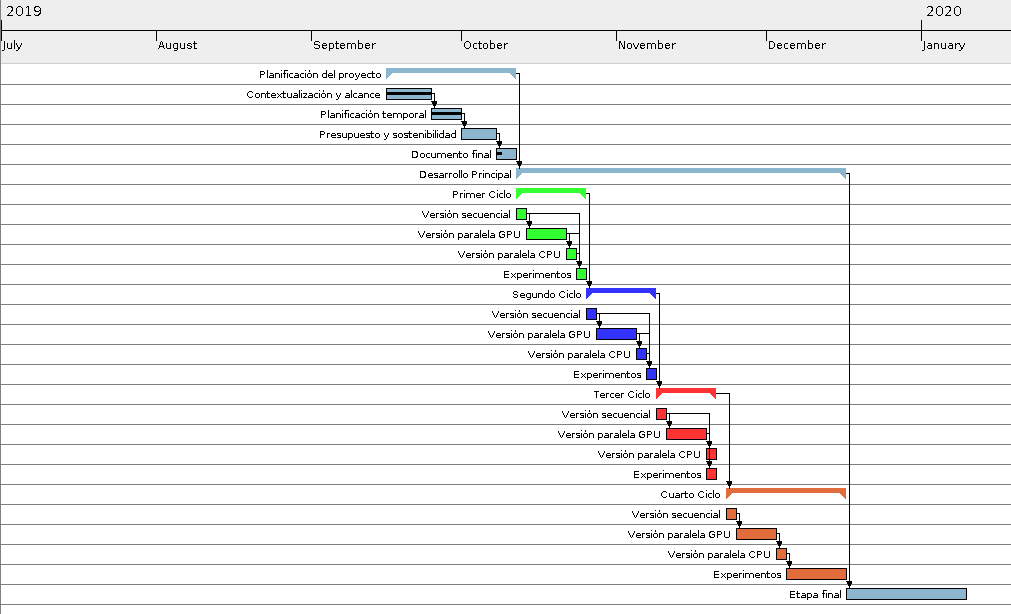
\includegraphics[scale=1.5]{media/gantt.png}
\captionof{figure}{Diagrama de Gannt completo. Fuente: Creación propia}
\label{gantt}
\end{figure}

\end{document}
